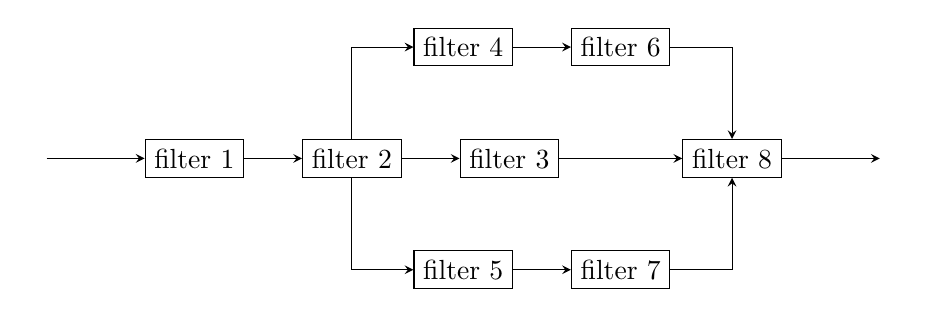
\begin{tikzpicture}[
>=stealth,
node distance=2cm,
arrow/.style={draw,->}
]

\node (empty) at (0,0) {};
\node[draw] (filter) [right of = empty] {filter 1};
\node[draw] (filter2) [right of = filter] {filter 2};
\node[draw] (filter3) [right of = filter2] {filter 3};
\node[draw] (filter4) [above right of = filter2] {filter 4};
\node[draw] (filter5) [below right of = filter2] {filter 5};
\node[draw] (filter6) [right of = filter4] {filter 6};
\node[draw] (filter7) [right of = filter5] {filter 7};
\node[draw] (filter8) [below right of = filter6] {filter 8};
\node (empty2) [right of = filter8] {};

\path[arrow] (empty) -- (filter);
\path[arrow] (filter) -- (filter2);
\path[arrow] (filter2) -- (filter3);
\path[arrow] (filter2) |- (filter4);
\path[arrow] (filter2) |- (filter5);
\path[arrow] (filter4) -- (filter6);
\path[arrow] (filter5) -- (filter7);
\path[arrow] (filter3) -- (filter8);
\path[arrow] (filter6) -| (filter8);
\path[arrow] (filter7) -| (filter8);
\path[arrow] (filter8) -- (empty2);

\end{tikzpicture}